\documentclass[../main.tex]{subfiles}

\begin{document}
    Das Spin-Hahn-Echo dient dazu die Kohärenz der einzelnen Spins aufrecht zu erhalten. Die Inkohärenz der Spins rührt aus Inhomogenitäten im Magnetfeld, die einzelne Spins aus dem \glqq{}Takt\grqq{} (genauer der Phase) geraten lassen. Um diesem Effekt vorzubeugen bzw. auszugleichen, wird nach dem \SI{90}{\degree}-Puls im zeitlichen Abstand $t_{e}$ ein \SI{180}{\degree}-Puls angelegt. Dieser sorgt für eine Verschiebung der Spins, wobei die schnelleren weiter zurückgeworfen werden, als die langsameren. So laufen die Spins wieder zusammen und der Phasenunterschied wird kleiner. Dieser Phasenunterschied wird über die $T_{2}^{*}$-Relaxationszeit gemessen. Es gilt 
    \begin{align}
        (T_{2}^{*})^{-1} = (T_{2})^{-1} + \gamma \Delta B_{0}
    \end{align}.
    


    
    
\end{document}

    \begin{figure}[h!]
        \centering
        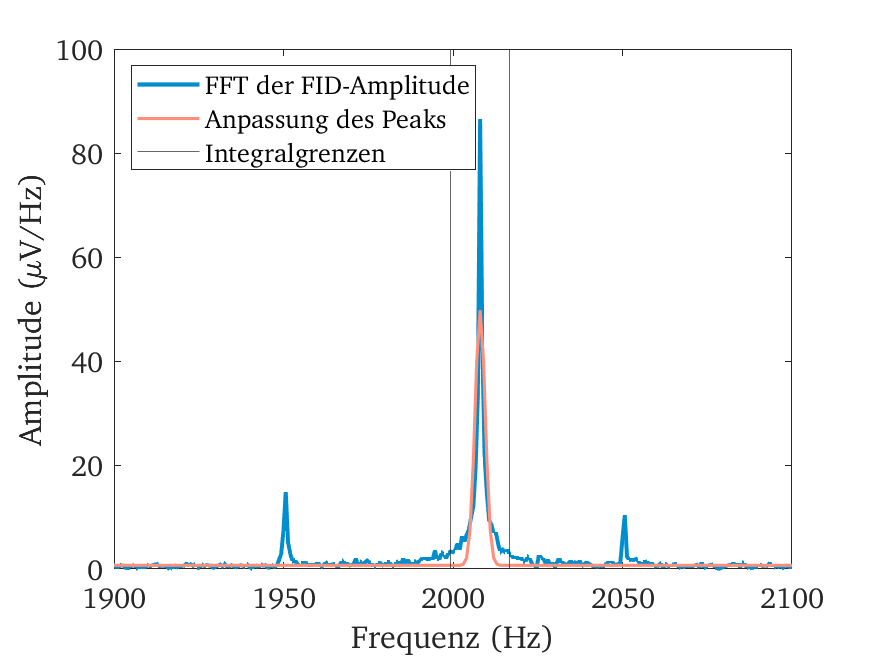
\includegraphics[width=\textwidth]{Bilddateien/7/Part7_Fig_2.png}
        \caption{Fouriertransformation des FID der Wasserflasche aus Abb. \ref{fig:FID_Optimised}.}
        \label{fig:FID_Optimised_FFT}
    \end{figure}